\documentclass[UTF8]{ctexart}
\usepackage{amsmath}
\usepackage{diagbox}
\usepackage{textcomp}
\usepackage{graphicx}
\usepackage{float}
\usepackage{caption}
\usepackage{adjustbox}
\usepackage{subfigure}
\usepackage{geometry}
\usepackage{pifont}
\usepackage{gensymb}
\usepackage{bm}
\usepackage{amstext}
\usepackage{amsfonts}
\usepackage{amssymb}
%引入代码块
\usepackage{listings}

\usepackage{xcolor}
%设置代码块格式

\definecolor{CPPGray}{RGB}{211,211,211}
\lstset{
 columns=fixed,       
 numbers=left,   % 在左侧显示行号
 numberstyle=\tiny\color{gray},% 设定行号格式
 frame=none,%none,% 不显示背景边框
 %aboveskip=1em,
 backgroundcolor=\color[RGB]{230,230,230},% 设定背景颜色
 keywordstyle=\color[RGB]{40,40,255},% 设定关键字颜色
 numberstyle=\footnotesize\color{darkgray},           
 commentstyle=\it\color[RGB]{0,96,96},% 设置代码注释的格式
 stringstyle=\rmfamily\slshape\color[RGB]{128,0,0},% 设置字符串格式
 showstringspaces=true,% 不显示字符串中的空格
 language=c++, % 设置语言
 morekeywords = {include,ull,int,double,return,static,typedef,if,else,for,long,void,class,struct,ll,while,do,throw,try,using,namespace,goto,switch,case,union,const},                % 自加新的关键字(必须前后都是空格)
}

\begin{document}
\renewcommand{\thefootnote}{\fnsymbol{footnote}}
\newgeometry{left=2cm,bottom=3cm,right=2cm}
\linespread{1.4}
\title{\vspace{-5em}\heiti平面上最近点对实验报告\vspace{-2.5em}}
\date{}
\maketitle
\begin{center}
{\fangsong 徐浩博\quad 软件02\quad2020010108}
\end{center}

\subsubsection*{摘要}
{\kaishu\normalsize  计算平面上最近点对的朴素做法的时间复杂度高达$n^2$,本实验试图描述一种$nlogn$复杂度的计算方法,并将运行时间与朴素做法进行比较. 最后,我还将此算法可视化,做到可以用鼠标输入和随机生成点两种输入方法,并计算出最近点对.}
\subsubsection*{关键词:最近点对\ \ 时间复杂度\ \ 程序可视化\ \ Qt\vspace{1.5em}}

\section*{1\ \ \ 实验环境}
操作系统:Windows 10\par
开发环境:Qt 5.15.2 MinGW 64-bit\par
处理器:Intel Core i7-10750H 六核CPU @ 2.60GHz\par
编程语言:C++11

\section*{2\ \ \ 算法分析}
\subsection*{2.1\ 暴力求解}
\paragraph{算法原理}\ \par
将n个点两两计算距离,总共需要计算$(n-1)+(n-2)+\cdots+1=n(n-1)/2$次距离,因此时间复杂度为$\Theta(n^2)$.\par
算法核心代码如下:

\begin{lstlisting}
    for (int i = 1; i <= n; i++){
		for (int j = i + 1; j <= n; j++){
			d = min(d, dist(point[i], point[j]))
		}
	}
\end{lstlisting}


\subsection*{2.2\ 分治求解}
事实上,我们可以考虑如下的分治方法:将点集$S$按照x坐标平分为两半(设分割线为midline),记为$S_1$和$S_2$,每一半各自求解点对距离最小值. 设$d({S})$为S内点对最小值,那么有:
\begin{equation}d(S)=\min\{d(S_1),\ \ d(S_2),\min_{u\in S_1,v\in S_2}dist(u,v)\}\end{equation}
分治法可以求解出$d(S_1),\ d(S_2)$;而将两个子问题合并时需要求解$\min\limits_{u\in S_1,v\in S_2}dist(u,v)$,下面的做法可以保证合并时时间复杂度为线性:\par
首先,如果$d(S)=\min\limits_{u\in S_1,v\in S_2}dist(u,v)$时,选取的点对的x坐标必然位于[midline - d,midline + d]中(其中$d=\min\{d(S_1),\ \ d(S_2)\}$,如果不如此则点对距离必然大于d,与假设矛盾);同理,点对的y坐标差值应该在[0,d]之间. 下面我们对于任意一个属于$S_1$且$x\in [midline - d,midline]$的点$u$考虑,如果$u$与之配对的$S_2$内的点$v$距离小于d,那么根据前面的推断,v必然位于下图的一个$d\times 2d$的矩形区域内. 
\begin{figure}[H]\begin{center}
	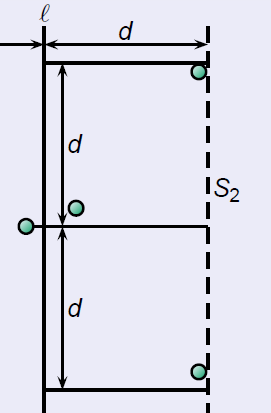
\includegraphics[scale = 0.5]{graph1.PNG}
\end{center}\end{figure}\par
更加细化后,我们发现该矩形区域内最多分布6个$v$备选点,且如下图中的小矩形区域所示,一个小区域最多一个备选点(反证法,如果一个区域有两个,那么它们之间的距离最大为对角线长度$5/6d<d$,与假设矛盾),因此对于每个$S_1$中的点$u$,我们只需按照y坐标看取与$u$坐标相近的上下六个点即可.\par
然而这里存在问题:如何找到与u的y坐标相近的点呢,为此我们可以在分治时,类似于归并排序,将点按照y坐标排序. 两个子集$S_1,\ S_2$内的点已经按照y单调排列,因此对于$S_1$内的点单调遍历,$S_2$中备选的六个点也是单调的;遍历后将两个y坐标排序数组合并即可.
\begin{figure}[H]\begin{center}
	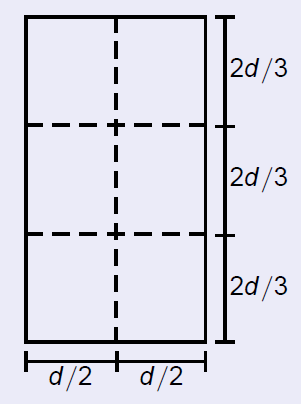
\includegraphics[scale = 0.5]{graph2.PNG}
\end{center}\end{figure}\par
考虑到分治分为两个小子问题,合并时时间复杂度为$\Theta(n)$,则有递推式$T(n)=2T(n/2)+\Theta(n)$,根据主定理,总时间复杂度为$O(nlogn)$.

\section*{3\ \ \ 运行时间比较}
为了比较二者的运行时间,我们将两个程序放置在一个cpp文件中,并且加上了随机生成数据的函数(详见".$\backslash$src$\backslash$RuntimeCompare"). 实验过程中取n=0$\sim$10000的情况,每隔$\Delta$n=200取样并记录运算时间,绘制成下图:
\begin{figure}[H]\begin{center}
	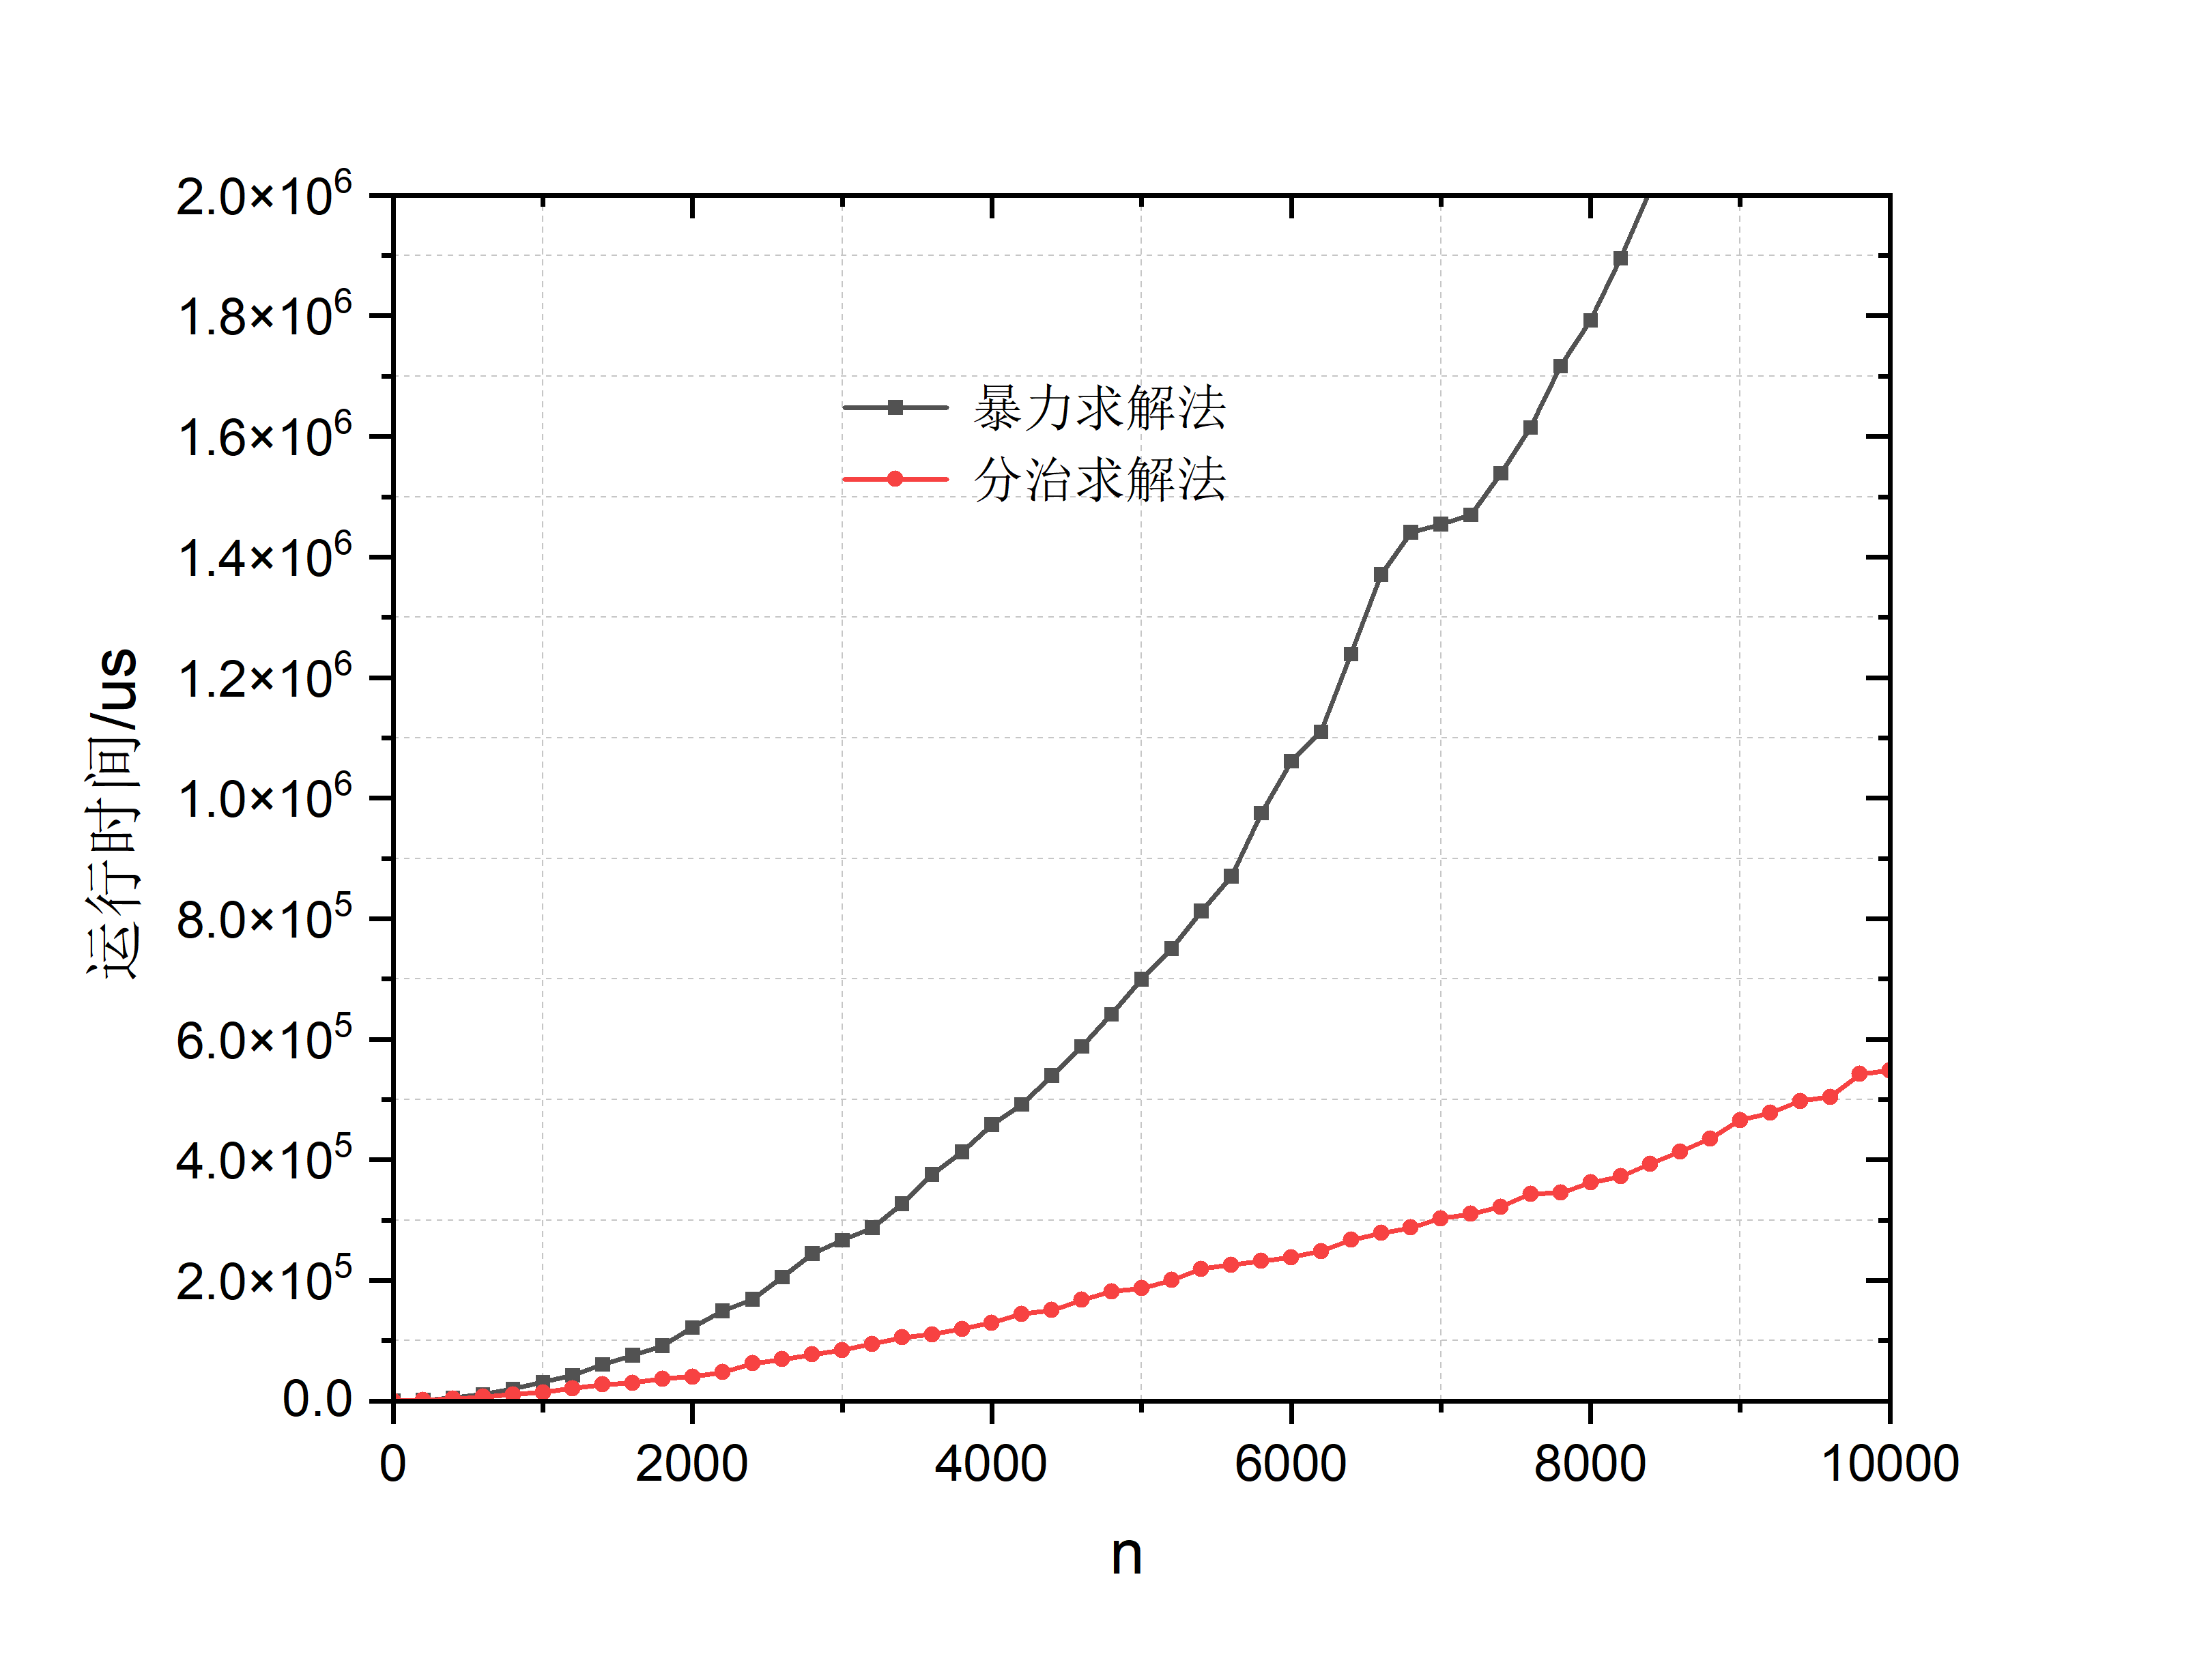
\includegraphics[scale = 0.5]{graph3.png}
\end{center}\end{figure}\par

我们可以明显看出,当数据规模较小时(n<=1000),暴力求解和分治算法运行时间十分接近;然而随着数据规模增大,暴力求解的运行时间增长得很快,而分治算法增长较为平缓. 时间复杂度$\Theta(n^2)$算法运行时间明显劣于$\Theta(nlogn)$算法.

\section*{4\ \ \ 可视化效果展示}
为了展现出可视化效果,我利用了Qt完成程序设计(详见".$\backslash$src$\backslash$qt"),效果展示如下:
\subsection*{4.1\ 主菜单}
程序主菜单如图:
\begin{figure}[H]\begin{center}
	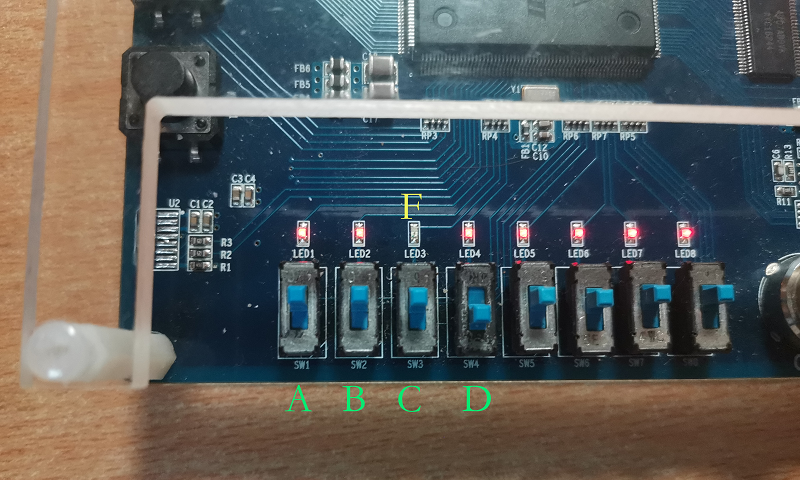
\includegraphics[scale = 0.5]{1.png}
\end{center}\end{figure}\par
按照按键指示可以分别体验程序的鼠标输入点和随机生成点两种功能.

\subsection*{4.2\ 鼠标绘制点并计算最近点对}
该功能主页面如图:
\begin{figure}[H]\begin{center}
	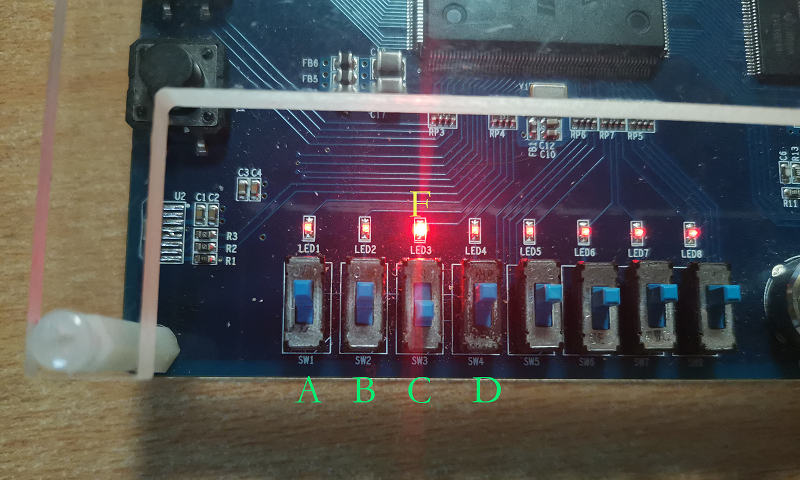
\includegraphics[scale = 0.5]{2.png}
\end{center}\end{figure}\par
鼠标在空白处单击即可生成点,待生成完毕后点击最左侧"开始计算"按键,则程序会计算最近点对并以红色标记标出,如下图:
\begin{figure}[H]\begin{center}
	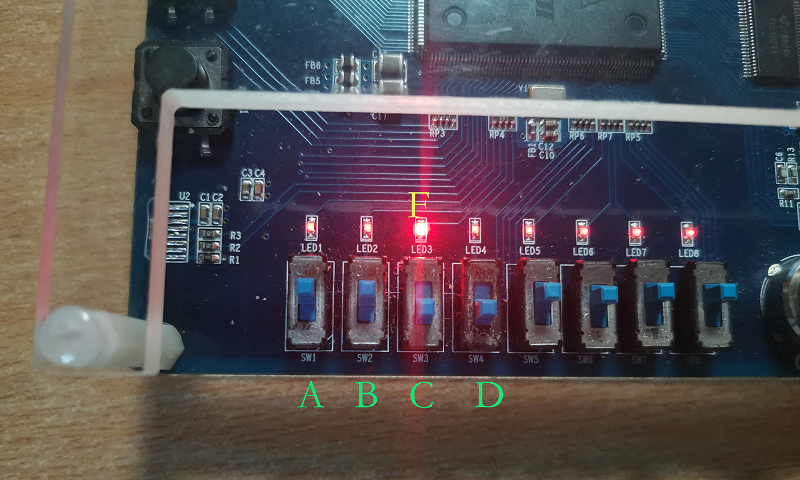
\includegraphics[scale = 0.5]{3.png}
\end{center}\end{figure}\par
计算最近点对后,可以选择继续点击空白生成点,抑或点击"重新绘制"清空已经绘制的点.

\subsection*{4.3\ 随机生成点并计算最近点对}
该功能主页面如图:
\begin{figure}[H]\begin{center}
	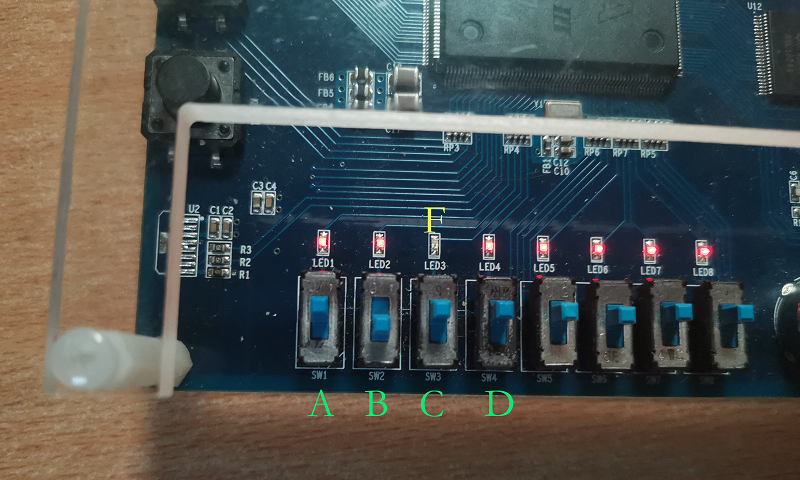
\includegraphics[scale = 0.5]{4.png}
\end{center}\end{figure}\par
在最上面的输入框中输入欲生成点的的个数n,点击"生成"随机生成n个点,同时自动计算出距离最近的点对的坐标和最近距离.
\subsection*{Problem 2}
我们假设事件$A_i$为$P[i]$与$P[1\sim(i-1)]$都不重复,题目所求即为$P(A_1A_2\cdots A_n)$,而$$
\begin{aligned}
P(A_1A_2\cdots A_n)&=P(A_1)P(A_2|A_1)P(A_3|A_2A_1)\cdots P(A_n|A_{n-1}\cdots A_1)\\
&=1\times\frac{n^3-1}{n^3}\times\frac{n^3-2}{n^3}\times\cdots\times\frac{n^3-(n-1)}{n^3}\\
&=1\times(1-\frac{1}{n^3})\times(1-\frac{2}{n^3})\times\cdots\times(1-\frac{n-1}{n^3})\\
&>(1-\frac{n}{n^3})^n\\
&=(1-\frac{1}{n^2})^n\\
&\ge 1-\frac{n}{n^2}=1-\frac{1}{n}
\end{aligned}$$\par
其中最后两行的推导运用了Bernoull不等式,即$(1+x)^n\ge 1+nx,\forall x>-1,n\ge 1$.\ $\blacksquare$
\end{document}
